% !TEX encoding = UTF-8 Unicode
%!TEX root = main.tex
% !TEX spellcheck = en-US
%%=========================================


%%%%%%%%%%%%%%%%%%%%%%%%%%%%%%%%%%%%%%%%%%%%%%%%%%%%%%%%%%%%%%%%%%%%%%%%%%%%%%%%
\chapter{Theoretical Background}
\label{ch:theoretical_background}


This chapter gives a more in\hyp{}depth explanation of different topics mentioned in the introduction, as well as other topics relevant to the thesis. These topics cover the required background knowledge, and each topic is presented on its own. The reader is encouraged to skim over this chapter, and rather come back and read more thoroughly when coming across a topic later in the thesis.


%%%%%%%%%%%%%%%%%%%%%%%%%%%%%%%%%%%%%%%%%%%%%%%%%%%%%%%%%%%%%%%%%%%%%%%%%%%%%%%%
\section{Concurrent Programming}
\label{sec:concurrent_programming}


Concurrent programming, or concurrent computing, is a form of computing to express programs or systems which execute multiple sequential computations in interleaving time periods, giving the impression of simultaneous execution. These computations are said to be running \textit{concurrently}, compared to \textit{sequentially} (one completing before the next start). These individual computations are often called \textit{processes} or \textit{threads}, which indicate a separate execution point. 

The notion of concurrency stems from the limitations of sequential programs and how all programs in the end is translated to machine code. Given the program is executed on a uniprocessor, only one machine code instruction will be executed at any given moment\footnote{Machine code execution is vastly more complex then presented here, e.g. pipelining and instruction\hyp{}level parallelism (ILP), but the sequential nature of program execution still stands}.  Since all computations in a sequential program must be executed sequential, it can be unintuitive how to model and implement systems which are inherently parallel. Concurrency aims to provide an abstraction level to bridge this limitation. Concurrent systems are therefore much more expressive than sequential systems, since it does not matter whether the program is executed in parallel or not, e.g. on a multiprocessor or uniprocessor.

It is important to note that concurrent programming is not the same as parallel programming. Concurrency is a form of abstraction, disregarding how the actual program execution is achieved. Parallelism refers to, in contrast to concurrency, the condition of a program being executed on multiple processors at once. One could therefore say that concurrency is possible on both uniprocessors and multiprocessors, while parallelism is only possible on multiprocessors.

Concurrency is a great tool for programmers, allowing concurrent systems to be expressed in a much more intuitive manner. It does however introduce an added mental overhead for the programmer, and is much more error\hyp{}prone compared to other types of programming paradigms. As a result, many programmers resort to other, less error\hyp{}prone programming paradigms than concurrent programming \citep{mordechai2006principles}.


%%%%%%%%%%%%%%%%%%%%%%%%%%%%%%%%%%%%%%%%
\subsection{Threading Models}
\label{subsec:threading_models}


Threading is the foundation of concurrency, which allows multiple computations to be executed simultaneously. Some sort of threading mechanism must be implemented on a platform to provide concurrency. On \textit{operating systems} (OS), threading mechanisms falls mainly into three types of threading models: \textit{user\hyp{}threads}, \textit{kernel\hyp{}threads}, or \textit{hybrid\hyp{}threads}, which is a combination of the two first models. \citet{c++csp2} goes into further detail on the three models, and a short summary is presented below.


%%%%%%%%%%%%%%%%%%%%%%%%%%%%%%%%%%%%%%%%
\subsubsection{User\hyp{}Threading}


User\hyp{}threads are a cooperative scheduling of threads executed in user space\footnote{Regarding operating systems, user space is a set of locations where normal user processes run}, and is called a \texttt{M:1} threading model. \texttt{M:1} means running \texttt{M} user\hyp{}threads on a single kernel\hyp{}thread. These user\hyp{}threads must cooperate on scheduling as the scheduling is non\hyp{}preemptive, meaning a running task is executed until completion or yields. Context switching and scheduling between these user\hyp{}threads is happening unbeknownst to the OS, resulting in much faster context switch times. This does however mean the OS cannot help with scheduling, and blocking calls in any user\hyp{}thread blocks all user\hyp{}threads on the given kernel\hyp{}thread. Only one user\hyp{}thread can run on a kernel\hyp{}thread at any time.


%%%%%%%%%%%%%%%%%%%%%%%%%%%%%%%%%%%%%%%%
\subsubsection{Kernel\hyp{}Threading}


Kernel\hyp{}threads are often directly supported in OS kernels and is called a \texttt{1:1} threading model. \texttt{1:1} means scheduling each kernel\hyp{}thread onto the available processors of the system. Kernel\hyp{}threads often use preemptive scheduling, meaning threads are given a priority, and the running thread is interrupted and later resumed whenever a thread with higher priority is ready. The OS is responsible for scheduling said threads. Kernel\hyp{}threads has no problems with blocking calls, as the OS can schedule any other kernel\hyp{}thread during a blocking call. Since the OS has full control over the scheduling it can much better utilize the available resources and time usage for each thread, compared to user\hyp{}threading. Context switching is however much slower than user\hyp{}threads because of overhead and kernel\hyp{}space\footnote{Regarding operating systems, kernel space is the location where the code of the kernel is stored and executed} crossing.


%%%%%%%%%%%%%%%%%%%%%%%%%%%%%%%%%%%%%%%%
\subsubsection{Hybrid\hyp{}Threading}


Hybrid\hyp{}threads is a combination of user\hyp{}threads and kernel\hyp{}threads, and is called a \texttt{M:N} threading model. \texttt{M:N} means running \texttt{M} user\hyp{}threads over \texttt{N} kernel\hyp{}threads. In other words, hybrid\hyp{}threading runs multiple kernel\hyp{}threads, with each kernel\hyp{}thread running multiple user\hyp{}threads. Blocking calls can still cause issues with unnecessarily blocking other user\hyp{}threads, but is possible to mitigate with running the blocking user\hyp{}thread on its own kernel\hyp{}thread. Scheduling user\hyp{}threads among the kernel\hyp{}threads can be much more difficult compared to user\hyp{}threading, as the OS cannot help with utilizing the available resources. 


%%%%%%%%%%%%%%%%%%%%%%%%%%%%%%%%%%%%%%%%
\subsection{Concurrency Concepts and Primitives}
\label{subsec:concepts_primitives}


Having multiple sequential executions running concurrently is not very useful if they cannot cooperate. Some form of interaction or communication between the computations must exist, which in turn requires coordination of access to shared resources. This coordination is called \textit{concurrency control}. Concurrency control means ensuring the correct and intended result from interactions between concurrent processes are upheld. 

To be able to manipulate shared resources safely requires introducing couple of new primitives and concepts. Below is a non\hyp{}exhaustive list of prevalent concurrency primitives presented.


%%%%%%%%%%%%%%%%%%%%%%%%%%%%%%%%%%%%%%%%
\subsubsection{Atomic Operations}


An operation is said to be \textit{atomic} or \textit{linearizable} if it appears to the rest of the system as instantaneous. In concurrent systems multiple processes can access the same shared resource at the same time. If one of the processes are changing the contents of a shared resource while another process is using the same resource, it is possible the operation results in an invalid or undefined state. It is obvious such situations requires atomic operations to force a linear sequence of well\hyp{}defined observable operations. 

Atomic operations exists both as low level and high level primitives. At the bottom we have processor instructions which are used to manipulate memory atomically. These usually include \textit{atomic read / write}, \textit{atomic swap}, \textit{test\hyp{}and\hyp{}set}, \textit{fetch\hyp{}and\hyp{}add}, \textit{compare\hyp{}and\hyp{}swap}, and \textit{load\hyp{}link / store\hyp{}conditional}. Modern processors usually support these types of instructions \citep{buck2009atomic}.

Further, these instructions are used to implement higher level primitives and non\hyp{}blocking algorithms. Examples of higher level primitive include semaphores, mutual exclusion locks, and monitors.


%%%%%%%%%%%%%%%%%%%%%%%%%%%%%%%%%%%%%%%%
\subsubsection{Critical Sections}


Concurrent access to shared resources can result in an invalid or undefined state, as stated above. Regions of code of which concurrent access by multiple processes where to cause erroneous behaviour are called \textit{critical sections} or \textit{critical regions}. These regions must therefore be protected by some sort of synchronization or lock mechanism. Critical sections usually accesses shared resources such as a data structures, IO operations or network sockets, where multiple concurrent access would result in incorrect behaviour \citep{raynal2012concurrent}.

Consider the following program: two processes, \texttt{A} and \texttt{B}, tries to respectively increment and decrement the shared resource \texttt{count} by one, initial value of $0$. See \cref{lst:critical_section_bad} for reference.

\begin{lstfloat}
\noindent\begin{minipage}{0.45\textwidth}
\begin{lstlisting}[title={Process A},style={CustomC},frame={},xleftmargin={4em}]
// Critical section
count = count + 1
\end{lstlisting}
\end{minipage}
\begin{minipage}{0.45\textwidth}
\begin{lstlisting}[title={Process B},style={CustomC},frame={},xleftmargin={4em}]
// Critical section
count = count - 1
\end{lstlisting}
\end{minipage}
\captionof{lstlisting}{Example of a critical section causing a race condition.}
\label{lst:critical_section_bad}
\end{lstfloat}

If both process \texttt{A} and \texttt{B} are executing the critical section at the same time, it is possible for the \texttt{count} resource to equal some whole number instead of the expected result $0$. This comes from the fact the incrementing and decrementing operations are not atomic operations, but a three\hyp{}stage operation of read\hyp{}modify\hyp{}write. 

If process \texttt{A} starts executing the increment, but is preempted before the write stage, process \texttt{B} can theoretically complete an arbitrary amount of decrement operations before process \texttt{A} is resumed. When process \texttt{A} is resumed, the old modified value of \texttt{count} is now written back instead of the updated value. This is a classic example of a \textit{race condition}, meaning the order and timing of which the operation is completed determines the outcome.

To achieve correct behaviour the critical section must be protected, usually done through some form of mutual exclusion. This consequently makes the critical section an atomic operation, as the read\hyp{}modify\hyp{}write operation is made indivisible to other processes.


%%%%%%%%%%%%%%%%%%%%%%%%%%%%%%%%%%%%%%%%
\subsubsection{Semaphores}


Semaphore is in software terms a data structure used to control access to a shared resource between multiple processes and to synchronize between processes. Invented by \citet{dijkstra}, and is one the simplest concurrency primitives used to build higher level concurrency control structures.

As described in \citet[chapter 2]{downey2016}, a semaphore is like an integer with three differences:

\begin{enumerate}[topsep=0em,itemsep=-1em,partopsep=0.5em,parsep=1em]
    \item When you create the semaphore, you can initialize its value to any integer, but after that the only operations you are allowed to perform are increment (increase by one) and decrement (decrease by one). You cannot read the current value of the semaphore.
    \item When a thread decrements the semaphore, if the result is negative, the thread blocks itself and cannot continue until another thread increments the semaphore.
    \item When a thread increments the semaphore, if there are other threads waiting, one of the waiting threads gets unblocked.
\end{enumerate}

Blocking in this sense means the scheduler will suspend the blocking thread until a corresponding event or operation which causes the thread to be unblocked. Both the increment and decrement operations are atomic, meaning multiple processes can concurrently access a semaphore.

Semaphores usually comes in two flavours: \textit{counting} and \textit{binary} semaphore. A counting semaphore allows an arbitrary resource count, while a binary semaphore allows only a resource count of $0$ and $1$ (hence the name binary). 

Semaphores are incredibly simple by definition, and are therefore often used to create more complex concurrency synchronization and structures. This includes structures such as \textit{locks}, \textit{monitors} and other \textit{synchronization patterns}. See \citet[chap. 3-7]{downey2016} for a more complete overview of such constructs.


%%%%%%%%%%%%%%%%%%%%%%%%%%%%%%%%%%%%%%%%
\subsubsection{Mutual Exclusion (Mutex)}


Mutual exclusion, \textit{mutex} for short, is used for protecting critical regions from concurrent access and to prevent race conditions. One can view mutexes as binary semaphores, with one important difference: mutexes has a notion of ownership. Only the process which was successful in acquiring the mutex can release it. 

Looking back at the example in \cref{lst:critical_section_bad}, wrapping a mutex around the critical section hinders process \texttt{A} and \texttt{B} of accessing the shared resource \texttt{count} simultaneously, and effectively turns the increment and decrement operation into an atomic operation. See \cref{lst:critical_section_good} for reference.

\begin{lstfloat}
\noindent\begin{minipage}{0.45\textwidth}
\begin{lstlisting}[title={Process A},style={CustomC},frame={},xleftmargin={4em}]
mutex.wait()
// Critical section
count = count + 1
mutex.signal()
\end{lstlisting}
\end{minipage}
\begin{minipage}{0.45\textwidth}
\begin{lstlisting}[title={Process B},style={CustomC},frame={},xleftmargin={4em}]
mutex.wait()
// Critical section
count = count - 1
mutex.signal()
\end{lstlisting}
\end{minipage}
\captionof{lstlisting}{A critical section surrounded by mutual exclusion, removing the race condition.}
\label{lst:critical_section_good}
\end{lstfloat}

Note that using mutual exclusion is very error prone, and might have unwanted side\hyp{}effects and conditions such as deadlocks, starvation and priority inversion. This is explained in further detail in \cref{subsec:common_pitfals}.


%%%%%%%%%%%%%%%%%%%%%%%%%%%%%%%%%%%%%%%%
\subsection{Common Pitfalls}
\label{subsec:common_pitfals}


As a consequence of using concurrency control, common pitfals and potential problems such as \textit{race conditions}, \textit{deadlocks}, \textit{livelocks}, \textit{starvation}, and \textit{priority inversion} must be taken into consideration. These are unwanted conditions or program states which are concurrent operations and interactions resulting in an erroneous state.


%%%%%%%%%%%%%%%%%%%%%%%%%%%%%%%%%%%%%%%%
\subsubsection{Race Condition}


As shown in \cref{lst:critical_section_bad}, race condition is when the output of an operation is dependent on the timing and sequence of other processes. Race conditions is never an intended behaviour of a program, as it is deemed undefined behaviour. This comes from the fact that the result of a race condition is the non\hyp{}deterministic result of timing between threads. 


%%%%%%%%%%%%%%%%%%%%%%%%%%%%%%%%%%%%%%%%
\subsubsection{Deadlock}


Deadlocks is a state in which a group of processes are each waiting for other members of the same group to release a lock, effectively halting progression. This is a direct consequence of enforcing mutual exclusion in critical sections. 

As described in \citet[page 239]{silberschatz2006operating}, a deadlock can only occur in a system if and only if all four of the \textit{Coffman conditions}\citep[First described][page 70]{coffman1971system} are held simultaneously. The conditions are as follows:

\begin{enumerate}[topsep=0em,itemsep=-1em,partopsep=0.5em,parsep=1em]
    \item \textit{Mutual exclusion} -- the resources involved must be unshareable.
    \item \textit{Hold and wait} -- a process holding at least one resource and requesting additional resources.
    \item \textit{No preemption} -- a resource can only be voluntarily released by the process holding it.
    \item \textit{Circular wait} -- each process must be waiting for a resource held by another process, which in turn is waiting for the first process to release the resource.
\end{enumerate}

There are several ways to handle deadlocks, but the three main approaches are \textit{ignoring}, \textit{detection} and \textit{prevention}. Ignoring is simply to assume a deadlock never occurs. Detection allows deadlocks to occur. If a deadlock is detected, the deadlock symmetry is broken by either terminating one or more of the deadlocked processes, or involuntarily preempt one or more of the deadlocked resources. Prevention is to simply prevent one of the four Coffman conditions from ever occurring.

The simplest example of a deadlock is the following scenario: two processes, \texttt{A} and \texttt{B}, tries to acquire two mutexes, \texttt{mutex\_A} and \texttt{mutex\_B}. Both processes acquires the mutexes in opposite order. A deadlock occurs when either process acquires its first lock, e.g. process \texttt{A} acquires \texttt{mutex\_A}, and is subsequently preempted. The other process is resumed and acquires its first mutex, e.g. process \texttt{B} acquires \texttt{mutex\_B}. Now when both processes tries to acquire its second mutex, both will promptly block forever, as both processes requires each other to release the mutex. A deadlock has now occurred. See \cref{lst:deadlock_example} for reference.

\begin{lstfloat}
\noindent\begin{minipage}{0.45\textwidth}
\begin{lstlisting}[title={Process A},style={CustomC},frame={},xleftmargin={4em}]
mutex_A.wait()
mutex_B.wait()
// some work
mutex_B.signal()
mutex_A.signal()
\end{lstlisting}
\end{minipage}
\begin{minipage}{0.45\textwidth}
\begin{lstlisting}[title={Process B},style={CustomC},frame={},xleftmargin={4em}]
mutex_B.wait()
mutex_A.wait()
// some work
mutex_A.signal()
mutex_B.signal()
\end{lstlisting}
\end{minipage}
\captionof{lstlisting}{Example of a simple deadlock between two processes.}
\label{lst:deadlock_example}
\end{lstfloat}

%%%%%%%%%%%%%%%%%%%%%%%%%%%%%%%%%%%%%%%%
\subsubsection{Livelock}


Livelock is similar to deadlock, as it is a state in which processes are not blocked, but are refrained from making progression. This can occur when processes are to busy responding to each other to resume work. 

Livelock is a rarer condition than deadlock, and can be harder to detect as the processes are not blocked when livelocked. 


%%%%%%%%%%%%%%%%%%%%%%%%%%%%%%%%%%%%%%%%
\subsubsection{Starvation}


Starvation is a condition where a process is denied further progress by perpetually being denied access to required resources or denied running time by higher priority processes. 

The absence of starvation in concurrent algorithms is called \textit{liveness}, which is a property guaranteeing all processes are able to make progress within finite time. 


%%%%%%%%%%%%%%%%%%%%%%%%%%%%%%%%%%%%%%%%
\subsubsection{Priority Inversion}


Priority inversion is a situation in scheduling where a higher priority process is indirectly preempted by a lower priority process, usually because of mutual exclusion. 

Consider the following example: process \texttt{H}, \texttt{M} and \texttt{L} has the priority ordering \texttt{p(H) > p(M) > p(L)}, and \texttt{H} and \texttt{L} both try to acquire the resource \texttt{R}. If \texttt{L} acquires the resource and is promptly preempted by \texttt{H}, \texttt{H} becomes blocked until \texttt{L} releases the resource. It is now possible for \texttt{M} to run over \texttt{L}, because of higher priority. Effectively \texttt{H} cannot run as \texttt{L} cannot release the resource, since \texttt{M} is preempting \texttt{L}. This is called \textit{priority inversion}. See \cref{fig:priority_inversion} for reference.

\begin{figure}[h!]
    \centering
    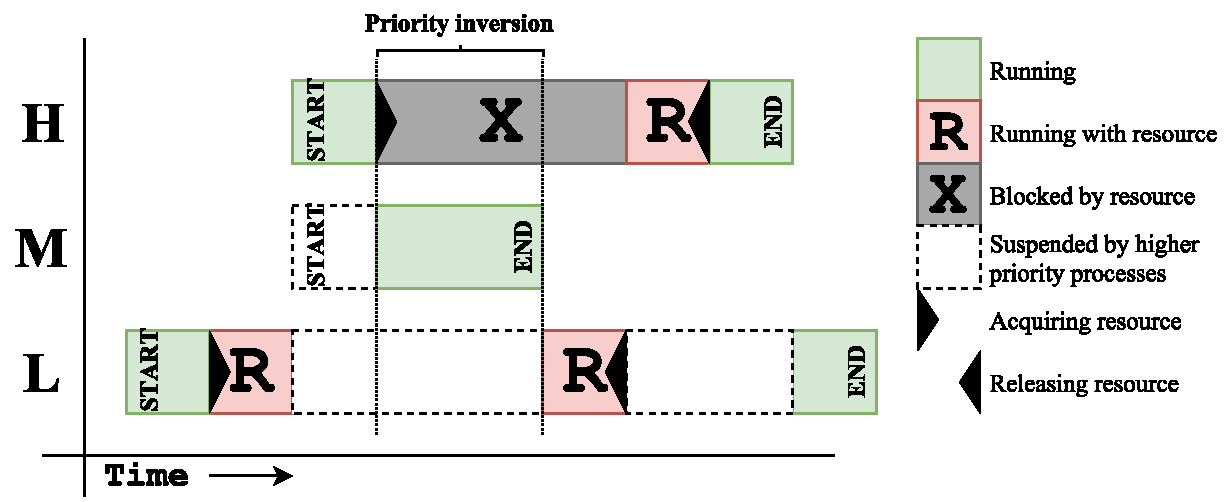
\includegraphics[width=0.9\linewidth]{fig/priority_inversion}
    \caption{Example of priority inversion with three processes.}
    \label{fig:priority_inversion}
\end{figure}

\textit{Bounded priority inversion} is when it can be proven priority inversion only occurs for a finite amount of time, while \textit{unbounded priority inversion} cannot prove this. 


%%%%%%%%%%%%%%%%%%%%%%%%%%%%%%%%%%%%%%%%%%%%%%%%%%%%%%%%%%%%%%%%%%%%%%%%%%%%%%%%
\section{Communicating Sequential Processes}
\label{sec:csp}


\textit{Communicating sequential processes} (CSP) is a mathematical formal language used in computer science to describe and model concurrent systems. First introduced by \citet{hoare1978communicating}, and was originally described as parallel composition of sequential disjoint processes with primitives for input and output, combined with guarded commands \citep{dijkstra1975guarded}. Communication was solely through message\hyp{}passing, which permitted synchronized communication between named processes.

Since its inception, CSP has undergone numerous transformations. As \citet{abdallah2005communicating} explains, most of the subsequent research has focused on a process algebra known as \textit{Theoretical CSP} (TCSP), which suppresses the imperative aspect of CSP \citep{brookes1984theory}. 

The strong points of CSP and TCSP is the ability to reason about correctness of the system being modeled. Since all communication between processes are limited to message\hyp{}passing, no primitive race conditions such as memory operations cannot occur. Further on, properties of the CSP models can be reasoned about, such as liveness, safety and deadlock.

In the industry, CSP is used to specify and verify the correctness of concurrent systems, especially communication and security protocols. The most prominent tool used is the \textit{failure\hyp{}divergence refinement} (FDR) checker \citep{manual2000failures}. FDR can statically prove if a concurrent system refines a given specification, has the correct liveness and safety properties, as well as absence of deadlocks and divergence. It is obvious such tools are powerful for systems that must prove its correctness before being deployed.

The ideas and expressiveness of CSP models has influenced the creation of concurrent programming languages, most notable occam \citep{inmos1988occam}, Ada \citep{ledgard1983reference}, XC \citep{douglas2009programming} and Go \citep{go2009go}. CSP frameworks has also been developed for programming languages which does not natively support CSP influenced concurrency, such as ProXC \citep{pettersen2016proxc} for C, C++CSP2 \citep{brown2007c++csp2} and CPPCSP \citep{chalmers2016cppcsp} for C++, JCSP \citep{welch2007jcsp} for Java, PyCSP \citep{bjorndalen2007pycsp} for Python, and much more.

It is understandable CSP is a great tool for concurrent systems. It provides a strong and safe framework for modelling and implementation, and allowing to prove the correctness of an implementation. This alleviates some of the mental overhead, as well as reducing the error prone nature of concurrent programming.


%%%%%%%%%%%%%%%%%%%%%%%%%%%%%%%%%%%%%%%%%%%%%%%%%%%%%%%%%%%%%%%%%%%%%%%%%%%%%%%%
\section{Memory Ordering}
\label{sec:memory_ordering}


Out of all CPU operations, memory accesses are among the slowest. Following Moore's law, CPU instruction performance has increased at a much greater rate than memory performance. Use of multilevel caches has been used to a great extent to bridge this gap in performance, however utilization of said caches could be improved. This is where \textit{memory reordering} comes in. To increase the performance of memory access further and properly utilize the hardware parallelism, memory operations can complete out of order \citep{mckenney2007memory}.

Several types of memory\hyp{}consistency models exist. \textit{Sequential consistency} is a guarantee that all processes agree on the order memory operations occur, even if they are completed out of order. The easiest configuration for sequential consistency is running all processes on a single core or a uniprocessor architecture. On multicore or multiprocessor architectures however, memory reordering can create inconsistencies between processes and proper care must therefore be taken to enforce correct memory ordering. 

There are different types of memory reordering, which usually falls into the categories of \textit{compiler reordering} and \textit{processor reordering}. As the name implies, compiler reordering is memory reordering done by the compiler at compile time, while processor reordering is memory reordering done by the processor at runtime.

Compiler reordering is obviously different from compiler to compiler, as it is implementation defined for each compiler. Processor reordering is also surprisingly different from CPU to CPU architecture. A \textit{memory model} is therefore used to describe what types of memory ordering to expect at runtime for a given processor, which again falls into the two categories \textit{weak} and \textit{strong} memory models.

As \citet{preshing2012weakstrong} explains it, a weak memory model can expect all types of memory reordering. This means any load or store operation can be reordered with any other load or store operation, and can reordered by both the compiler or processor. In contrast, a strong memory model limits the types of memory reordering. More specifically, only \texttt{store\hyp{}load} reordering is permitted. 

To enforce correct memory ordering, some type of \textit{memory barrier} must be used \citep{preshing2012barriers,preshing2012lockfree}. These exists as both software and hardware semantics, and are generally implemented as some sort of \textit{acquire} and \textit{release} semantics \citep{preshing2012acquire}.

Memory ordering is important to take into consideration when creating non\hyp{}blocking algorithms, as the memory operations in critical regions must have a sequential consistency between processors. More of this explained in \cref{sec:nonblocking_algorithms}.


%%%%%%%%%%%%%%%%%%%%%%%%%%%%%%%%%%%%%%%%%%%%%%%%%%%%%%%%%%%%%%%%%%%%%%%%%%%%%%%%
\section{Non\hyp{}Blocking Algorithms}
\label{sec:nonblocking_algorithms}


To fully utilize multiprocessors, most programs are multiprogrammed. Preemptive multiprocessor operating systems has the unfortunate effect of degrading performance in synchronized parallel programs if the preemption is ill\hyp{}timed, and access to shared data structures is usually the root of the cause. As \citet{michael1998nonblocking} explains, these data structures needs to ensure concurrent access is consistent and well\hyp{}formed across processes, which is usually implemented by protecting critical sections with mutual exclusion. Mutual exclusion locks does not scale well in performance on time\hyp{}sliced multiprogrammed systems \citep{zahorjan1991effect} due to preemption of processes holding locks. The preempted process must be rescheduled and release the lock before any waiting processes can progress.

One principal strategy to mitigate ill\hyp{}timed preemptions are \textit{non\hyp{}blocking algorithms}. Non\hyp{}blocking algorithms has the property any process cannot cause failure nor suspension of any other process, despite failures or suspension of itself. Two types of guarantees are usually associated with nonblocking algorithms to describe how strong this property is: \textit{lock\hyp{}free} and \textit{wait\hyp{}free}. 

Lock\hyp{}freedom guarantees system\hyp{}wide progress, and can be defined as: given a meaningful definition of progress, an algorithm is lock\hyp{}free if at least one process in a program makes progress if all processes are given sufficient running time. Wait\hyp{}freedom guarantees process\hyp{}wide progress, and can be defined as: an algorithm is wait\hyp{}free if every operation in the algorithm has an upper bound of computational time before it completes. Wait\hyp{}freedom implies lock\hyp{}freedom, which makes wait\hyp{}freedom a stronger guarantee than lock\hyp{}freedom.

\citet{preshing2012lockfree} describes the \textit{lock} part of non\hyp{}blocking algorithms (or as lock\hyp{}free programming he refers it to) as ``the possibility of "locking up" the entire application in some way, wheth\-er it's deadlock, livelock -- or even due to hypothetical thread scheduling decisions made by your worst enemy''. This means code not containing any locks, such as mutexes, may still not be lock\hyp{}free. 

It is rare a concurrent program is entirely lock\hyp{}free or wait\hyp{}free, which is why the focus is on non\hyp{}blocking algorithms rather than non\hyp{}blocking programs. Generally, a set of high contention operations between processes are set out to be non\hyp{}blocking, such as access and manipulation to shared data structures.

A handful of techniques are used to implement non\hyp{}blocking algorithms, most commonly a combination of atomic operations, memory barriers and general patterns. While the atomic primitives \texttt{read\hyp{}modify\hyp{}write} and \texttt{compare\hyp{}and\hyp{}swap} forms the basis of most non\hyp{}blocking algorithms, memory models and memory ordering needs to be taken into consideration as well. Since different processors have different memory models, it is not given processes agree on the order in which memory operations occur. Memory reordering can cause memory inconsistencies between processes, which is why sequential consistency or memory barriers are needed, especially on multicore architectures \citep{preshing2012weakstrong,preshing2012barriers,preshing2012lockfree,preshing2012acquire}.


%%%%%%%%%%%%%%%%%%%%%%%%%%%%%%%%%%%%%%%%%%%%%%%%%%%%%%%%%%%%%%%%%%%%%%%%%%%%%%%%
\section{Dynamic Multithreading}
\label{sec:dynamic_multithreading}


Getting the potential performance out of multicore processors requires fully utilizing the available processor cores. Amdahl's law \citep{amdahl1967validity} argues that the maximum potential speedup in a program with infinite number of parallel processors is limited to $^1/_s$, given the fraction of sequential work in the program is $s$. Because of Ahmdal's law, multiprogrammed concurrent programs needs to identify the potential parallelism and convert sequential work into parallel work to exploit multicore performance. This responsibility is mostly up to the programmer to identify, and in most cases is easier said than done. Simple constructs such as loops and loosely coupled sections are easy to detect and convert \citep{dagum1998openmp,robison2013composable}, but a program\hyp{}wide parallelism is far from intuitive to detect and how to schedule such parallelism effectively on multicore processors. 

\textit{Dynamic multithreading} is a strategy to abstract away the scheduling and instead focus on detecting the units of parallel work in the program. The idea is letting the program spawn and synchronize new processes or tasks which executes some kind of computation, and some sort of runtime takes care of the scheduling.

Based on the threading models (see \cref{subsec:threading_models}) the naïve approach would be spawning kernel\hyp{}threads for each process. The operating system is responsible for creating, scheduling and destroying the processes, as well as scheduling the processes among the available cores. However, kernel\hyp{}threads are expensive to create, context switching between kernel\hyp{}threads are relative slow, and scales very badly in performance with an increase in kernel\hyp{}threads running simultaneously. This severely limits the use of processes, and makes it very unintuitive on how to distribute the parallel work efficiently.

Using hybrid\hyp{}threads, a combination of user\hyp{}threads running on multiple kernel\hyp{}threads, is an improvement on only kernel\hyp{}threads. Each spawned process is a user\hyp{}thread, scheduled on a static number of kernel\hyp{}threads equal to the number of available cores. User\hyp{}threads are much cheaper to create, context switching is relatively much faster, and scales much better performance wise. The problem is how to efficiently schedule and distribute these processes between the available kernel\hyp{}threads, since an intermediate runtime environment has to exist between the user\hyp{}threads and the operating system.

Two principal scheduling strategies exist to efficiently distribute and schedule processes among a static number of kernel\hyp{}threads, namely \textit{work stealing} and \textit{work sharing}.


%%%%%%%%%%%%%%%%%%%%%%%%%%%%%%%%%%%%%%%%
\subsection{Work Stealing}
\label{subsec:work_stealing}


Given a processor with $P$ cores, $P$ kernel\hyp{}threads are created with each running a scheduler. Each scheduler has a pool of ready work. Whenever a schedule runs out of ready work, it selects another scheduler (called victim) and tries to steal work. If the steal was successful, it continues the stolen work. Spawning processes simply pushes the spawned process in the ready pool \citep{blumofe1999scheduling}.

Different types of work stealing algorithms exist, but the main emphasis is on the victim selection and stealing procedure. The most popular algorithm is the randomized work stealing algorithm first detailed in \citet{blumofe1999scheduling}. Whenever a scheduler is empty for ready work, a victim is chosen uniformly at random. If the victims ready pool is not empty, try to steal work. If successful, resume said work, else start over the selection procedure.

The most common way to represent ready work is by using a double\hyp{}ended queue, or \textit{deque} for short, where the ends of the deque is called \textit{top} and \textit{bottom}. The scheduler owning the deque has access to the bottom of the deque, where it can push and pop ready work. Any other schedulers can try to steal from the top of the deque if it is non\hyp{}empty. Much research has gone into creating these deques as efficient and low overhead as possible \citep{chase2005dynamic,le2013correct}, as they can be high contention area between kernel\hyp{}threads.

Many runtime frameworks for dynamic parallel computations has been created with work stealing \citep{blumofe1996cilk,sunderam1990pvm}, and with great success performance wise.


%%%%%%%%%%%%%%%%%%%%%%%%%%%%%%%%%%%%%%%%
\subsection{Work Sharing}
\label{subsec:work_sharing}


As the same setup as work stealing, $P$ kernel\hyp{}threads are created on a processor with $P$ cores with each running a scheduler. The big contrast to work stealing is work sharing manually distributes each work among the schedulers whenever new work is spawned. 

Usually work stealing is preferred over work sharing, as work stealing causes less process migration between schedulers. As \citet[page 721]{blumofe1999scheduling} argues, ``Intuitively, the migration of threads occurs less frequently with work stealing than with work sharing, since when all processors have work to do, no threads are migrated by a work stealing scheduler, but threads are always migrated by a work sharing scheduler''.

